% Generated from 19-开源生态、代码库与工具链.md; edit the LaTeX source after migration.

\part*{第十九部分 开源生态、代码库与工具链}
\addcontentsline{toc}{part}{第十九部分 开源生态、代码库与工具链}
\markboth{第十九部分 开源生态、代码库与工具链}{第十九部分 开源生态、代码库与工具链}

具身智能领域的开源生态与纯软件 AI 有一个明显不同：它不仅包含模型代码，还包含数据格式、机器人接口、仿真环境、评测协议和部署工具。也正因为如此，开源生态在机器人领域既是研究扩散器，也是能力过滤器。一个方向若没有开源支撑，研究社区很难充分比较；但即使开源存在，也不代表该路线足够接近真实部署。

更准确地说，具身开源生态不是一个平面的“代码仓库集合”，而是一套层层嵌套的基础设施：上游有视觉 backbone、自监督表征与通用训练框架；中游有机器人策略模型、数据格式、仿真与 benchmark；下游还有数据采集、日志回放、边缘推理、部署监控和 ROS/中间件接口。理解这个生态时，最重要的不是“哪个仓库最火”，而是它在这条链路上处于哪个位置，以及它暴露了多少真实系统假设。

\chapter*{91. 开源模型}
\addcontentsline{toc}{chapter}{91. 开源模型}
\markboth{91. 开源模型}{91. 开源模型}

\section*{91.1 机器人基础模型}
\addcontentsline{toc}{section}{91.1 机器人基础模型}


因此，阅读这类项目时最值得优先检查的通常是四件事：数据接口是否公开、动作表示是否明确、评测脚本是否可复现、部署约束是否被说明。只有这四项同时透明，基础模型才真正具备被社区继承和审查的价值。否则，它更像一个展示研究方向的样板，而不是一套可积累的公共资产。 把“机器人基础模型”作为开源生态中的一类对象单列出来，是因为它们往往不只是一个 checkpoint，而是一整套关于数据接口、动作表示、多任务条件化和评测方法的默认设定。对学习者而言，看这类项目时最重要的不是先问“参数有多大”，而是先问“它假设机器人问题该被怎样组织”。 但评价这类开源基础模型时，不能只看“是否开源了权重或代码”，还要看它是否把训练接口、动作表示、数据协议和评测脚本同时开放出来。对机器人来说，单独公开一个 checkpoint 的价值有限，因为真正决定复现与迁移成本的，往往是数据切片逻辑、动作 token 化方式、传感输入规范和与执行栈的绑定关系。也正因如此，能够把这些接口一并暴露出来的项目，往往比单点模型开源更有长期研究价值。

从学习路径上看，这类项目最适合承担“读懂问题设定”的功能，而不一定最适合直接变成你的第一套可部署系统。也就是说，它们往往更像研究接口样板，而不是现成产品模板。

OpenVLA 等项目的重要性，在于它们首次让研究者更系统地观察 VLA 路线的训练与部署接口，而不是只能依赖闭源演示理解其能力边界。\href{https://arxiv.org/abs/2406.09246}{OpenVLA}

我更建议把“机器人基础模型开源度”再拆成三层来看。第一层是论文级开放，只告诉你模型大致结构；第二层是代码/权重级开放，让你能真正复现实验；第三层是协议级开放，把数据 schema、动作表示、评测脚本、适配方法和部署入口一起公开。只有到第三层，项目才更接近可继承基础设施。像 \href{https://github.com/openvla/openvla}{OpenVLA GitHub} 这种同时公开模型、数据接口、微调与服务化入口的项目，和只给 checkpoint 或演示脚本的项目，研究价值并不在同一个数量级上。

\section*{91.2 policy 学习模型}
\addcontentsline{toc}{section}{91.2 policy 学习模型}


policy 学习模型这一类开源项目的真正价值，在于它们把机器人动作生成问题变成可直接替换、比较和复用的研究接口。不同仓库虽然名字各异，但常常围绕同几类分歧展开：动作是回归、扩散还是 token；输入窗口多长；是否支持多任务；是否显式建模恢复或闭环重规划。 这一类开源 policy 项目的真正意义，是把机器人动作学习从“彼此难以比较的私有实验”逐步推进成“至少在接口层可互译的研究对象”。它们提供的不只是算法实现，更是一套默认问题设定：观测窗口如何构造、动作是逐步输出还是 chunk 输出、损失函数如何兼顾平滑性与目标完成、评测时是否允许重规划。换句话说，policy 开源生态实际上在不断塑造研究共同体默认承认什么叫“可比较的动作学习结果”。

对报告维护者而言，这意味着后续每看到一个新 policy 仓库，都应先判断它是在重写哪一层默认设定，而不是只记录“又多了一个新模型名”。只要把这一习惯固定下来，第 19 章就不会沦为仓库名单。

这些工作为更通用的策略学习提供了基线，使动作生成、轨迹建模和条件化策略学习得以进入更统一的比较框架。代表性论文可参见 \href{https://arxiv.org/abs/2303.04137}{Diffusion Policy：扩散式机器人策略}、\href{https://arxiv.org/abs/2106.01345}{Decision Transformer：序列化决策} 与 \href{https://arxiv.org/abs/2304.13705}{ACT：动作块 Transformer}。

如果把这一类开源 policy 按“动作是怎样被组织出来的”来分层，至少可以得到四类主流写法。第一类是\texttt{\detokenize{自回归序列策略}}，其典型形式更接近

\begin{equation*}
p(a_t \mid o_{\le t}, a_{<t}, g)
\end{equation*}

即把决策写成条件序列建模问题，\href{https://arxiv.org/abs/2106.01345}{Decision Transformer：序列化决策模型} 是这一思想在决策领域的经典入口。第二类是\texttt{\detokenize{动作块策略}}，直接预测未来 \(H\) 步动作片段，

\begin{equation*}
p(a_{t:t+H-1} \mid o_{\le t}, g)
\end{equation*}

这样做的好处是减少逐步解码抖动，\href{https://arxiv.org/abs/2304.13705}{ACT：动作块 Transformer} 就把“动作块”明确写成策略接口。第三类是\texttt{\detokenize{扩散式动作策略}}，以迭代去噪方式生成动作序列，\href{https://arxiv.org/abs/2303.04137}{Diffusion Policy：扩散式机器人策略} 代表了这种路线，其优势在于对多峰动作分布的刻画能力更强。第四类则是\texttt{\detokenize{通用策略底座 + 跨本体数据协议}}路线，例如 \href{https://arxiv.org/abs/2405.12213}{Octo：开源通用机器人策略}、\href{https://arxiv.org/abs/2406.09246}{OpenVLA：开放视觉-语言-动作模型} 与 \href{https://arxiv.org/abs/2310.08864}{Open X-Embodiment：跨本体机器人数据开放协议} 所共同推动的方向：不再只优化单一本体上的策略拟合，而是把动作接口、数据模式与迁移方式一起做成生态对象。

因此，读一个开源策略项目时，至少应先看四个维度。第一是\texttt{\detokenize{动作表示}}：到底输出单步连续动作、动作块、离散动作记号还是技能索引。第二是\texttt{\detokenize{时间抽象}}：它是在毫秒级控制上出动作，还是在较低频率上出未来一段动作计划。第三是\texttt{\detokenize{跨本体适配方式}}：它假设所有机器人共享同一动作语义，还是允许通过适配器、归一化和数据模式映射来组织差异。第四是\texttt{\detokenize{运行时接口}}：模型训练出来之后，是只停留在笔记本实验或离线展开脚本，还是已经暴露推理服务、机器人适配、日志和回放接口。只要这四维被看清，一个策略仓库的研究位置就会比“代码托管平台热度高不高”更明确。

从这个角度看，policy 开源项目还可以进一步分成三类资产。\texttt{\detokenize{研究样本}}主要公开论文对应实现，用于说明方法是否成立；\texttt{\detokenize{系统样本}}开始把数据处理、评测和部署入口一起暴露出来，用于说明方法如何接进真实软件栈；\texttt{\detokenize{基础设施样本}}则进一步把数据 schema、训练脚本、机器人适配、回放和运行时服务都稳定公开，使后来者可以在其上持续叠加。像 \href{https://github.com/openvla/openvla}{OpenVLA GitHub} 与 \href{https://github.com/huggingface/lerobot}{LeRobot GitHub} 之所以值得长期跟踪，正是因为它们开始显式提供第二类甚至向第三类过渡的资产，而不只是“模型权重下载入口”。

同样重要的是，要把失败模式一起写进阅读框架。当前开源 policy 最常见的四类脆弱点是：第一，\texttt{\detokenize{恢复盲区}}，即模型擅长主路径模仿，却缺少失败后回退与二次尝试能力；第二，\texttt{\detokenize{动作接口错配}}，即离线动作格式与真实控制器消费接口不一致；第三，\texttt{\detokenize{时延敏感性}}，即模型在离线 rollout 中表现良好，但在边缘设备或网络链路上推理抖动明显；第四，\texttt{\detokenize{跨本体幻觉}}，即表面上支持多机器人训练，实际上控制频率、夹具和示教语义并未真正对齐。只要这些问题没有被公开处理，再漂亮的开源 policy 也更接近“研究现象样本”而不是“可继承工程资产”。

对后续版本维护而言，这一节最值得固定成纪律的不是项目名单，而是一条阅读顺序：

\begin{enumerate}
\item 先看数据协议：这个 policy 默认读取什么 schema、什么时间切片、什么动作语义。
\item 再看动作表示：它输出单步、chunk、token 还是技能。
\item 再看评测协议：它的 benchmark 到底奖励主路径命中、恢复能力还是长时稳定性。
\item 最后看运行时接口：它是否真正暴露服务化、日志、适配和回退入口。
\end{enumerate}

只要沿着这条顺序去读，新项目就更不容易把我们重新拉回“仓库很热所以路线很重要”的浅层判断。

\section*{91.3 多模态与世界模型相关开源项目}
\addcontentsline{toc}{section}{91.3 多模态与世界模型相关开源项目}


这一类项目的真正价值，在于它们虽然不一定直接输出机器人动作，却经常决定机器人系统能带着什么样的表征先验进入训练。视觉 backbone、自监督表示学习库、视频预测框架和多模态训练基座，往往在机器人专用仓库之前就已经改写了输入表示、时间建模方式和跨模态对齐接口。若只盯着最下游 policy 仓库，读者很容易错过这些更高杠杆的变化。

因此，更稳妥的阅读方法不是把它们视为“外围材料”，而是把它们放进同一条具身软件栈里理解：上游项目决定先验与表示，中游项目决定动作建模接口，下游项目决定评测与部署可行性。只有建立这种分层视角，开源生态才会从零散仓库收藏夹，变成可复用的研究地图。 这类项目的重要性，在于它们虽然不一定直接输出机器人动作，却决定了机器人上游表征、视频预测、抽象状态建模和多模态对齐能力的边界。很多机器人基础模型表面属于“机器人代码库”，底层却大量复用这些更通用的多模态资产。 这类项目常常不是直接面向机器人部署，却对后续具身路线产生上游决定性影响。很多机器人基础模型表面上是“机器人论文”，底层却大量借用了视觉 backbone、视频预测模型、自监督表征学习库和通用多模态训练框架。因而研究者若只跟踪机器人专属仓库，很容易错过真正改变接口能力的上游变化。理解开源生态时，必须把“机器人项目”与“机器人所依赖的通用表征资产”放在同一张图里。

世界模型、感知 backbone、自监督表示学习和视频预测的开源实现，则为后续机器人基础模型提供了大量上游组件。很多“机器人模型”真正依赖的，其实是这些更一般的开源表示学习资产。

这提醒我们在阅读机器人开源项目时，不应只盯着最下游 policy 仓库。很多决定系统上限的变化，其实先发生在上游视觉、自监督、多模态和视频建模资产中，而机器人仓库只是把这些能力重新绑到动作接口上。

\section*{91.4 轻量化与端侧路线的开源意义}
\addcontentsline{toc}{section}{91.4 轻量化与端侧路线的开源意义}


轻量化开源路线还有一个经常被忽视的价值：它更早暴露真实部署约束。大模型演示往往默认充足算力、干净网络和高成本硬件，而轻量化项目会迫使社区正视模型尺寸、推理时延、内存占用、热设计功耗和设备成本这些不浪漫却决定落地成败的问题。因此，这类路线虽然在“能力想象空间”上不如巨型模型耀眼，但在“什么东西真正能在机器人上跑起来”这件事上，往往更接近现实。

SmolVLA、LeRobot 等路线之所以值得跟踪，不只是因为它们“能跑在更小机器上”，而是因为它们把低成本复现、社区参与和端侧约束一起变成研究目标。这与只发布一个大模型 checkpoint 的意义完全不同。\href{https://arxiv.org/abs/2506.01844}{SmolVLA}、\href{https://arxiv.org/abs/2602.22818}{LeRobot}

这类路线还有一个研究方法上的额外价值：它们迫使社区把“真实机器人算力预算”重新写回实验设计。过去很多研究默认离线训练与在线推理的资源约束完全不同，因此模型结构可以任意膨胀；而轻量化路线会逼迫研究者重新回答几个不那么浪漫但极其关键的问题：

\begin{enumerate}
\item 模型能否在板载设备稳定运行。
\item 量化、蒸馏与裁剪是否会破坏动作稳定性。
\item 端侧延迟抖动会不会直接影响闭环控制。
\item 小模型是否仍然保留足够的恢复与重试能力。
\end{enumerate}

也因此，轻量化开源项目的价值常常不在于“指标最强”，而在于它们更早暴露出哪些能力是真正可以被部署继承的，哪些能力只是靠高算力实验环境暂时堆出来的。

这一层近两年最值得重视的变化，是轻量化项目不再只发布“压缩版模型”，而开始把低门槛硬件、统一数据格式和最小复现实验一起交给社区。\href{https://github.com/huggingface/lerobot}{LeRobot} 明确把真实机器人训练、评测、遥操作、低成本机械臂与硬件无关接口放进同一项目叙事；\href{https://arxiv.org/abs/2506.01844}{SmolVLA} 则把“小模型也要保留真实机器人可用性”作为正式研究目标。这说明端侧开源路线的价值，已经从“给弱设备一个替代品”升级成“把真实部署约束重新写回研究默认设定”。

\chapter*{92. 开源数据集与 benchmark}
\addcontentsline{toc}{chapter}{92. 开源数据集与 benchmark}
\markboth{92. 开源数据集与 benchmark}{92. 开源数据集与 benchmark}

\section*{92.1 操作数据集}
\addcontentsline{toc}{section}{92.1 操作数据集}


操作数据集最容易被误读的地方，是外界常常只盯着轨迹条数或任务数量，却忽略了协议层质量。对具身模型而言，更关键的问题往往是：动作空间是否一致，传感器与控制时间轴是否对齐，失败样本是否被完整保留，episode 边界如何定义，任务标签是否稳定，元数据能否支持跨任务重采样。这些看起来“工程化”的细节，往往比样本总量更决定可学性。

也因此，一个真正高价值的操作数据集，通常不只是数据文件本身，还包括清洗脚本、对齐规则、重采样工具、成功判定协议和版本化维护方法。若这些内容缺失，再大的数据池也可能很难转化成稳定的监督资源。 操作数据集之所以要单列，是因为它们定义了机器人“如何被看作一个训练样本生成器”。一个好的操作数据集不仅要有成功轨迹，还要有清晰动作接口、时间同步、失败样本、任务标签和足够可解释的元数据。 对操作数据集的判断也不能停留在“规模大不大”。真正关键的是它是否清楚定义了动作接口、对齐了传感与控制时间轴、覆盖了多少失败样本，以及任务成功究竟是以什么标准标注。一个看起来规模不小的数据集，如果动作协议混乱、示教质量不均或失败片段被大量过滤掉，最后很可能更适合做演示型模仿，而不适合做稳健闭环学习。

Open X-Embodiment 的重要性在于它尝试把跨平台机器人数据组织成可比较接口，这是机器人数据工程走向基础模型的关键一步，相关论文可参见 \href{https://arxiv.org/abs/2310.08864}{《Open X-Embodiment》}。

\section*{92.2 导航与移动数据集}
\addcontentsline{toc}{section}{92.2 导航与移动数据集}


导航与移动数据集的价值，在于它们更早把长期任务、地图记忆、重定位和场景级评测问题组织成了较成熟的 benchmark 传统。对具身学习者来说，这类传统很有借鉴意义，因为它说明：很多看似“新”的长时程问题，其实早已在移动机器人与 embodied AI 里被系统化处理过。 导航数据集和 benchmark 的长期价值，在于它们更早积累了“场景级结构化评测”传统。这类传统对具身智能很重要，因为它提醒我们：真正困难的问题往往不在单步感知，而在长时程任务中如何处理记忆、重定位、地图误差和恢复。也正因如此，导航生态里那些关于 episode 定义、重置条件、成功半径和探索预算的设计经验，后来都对更广义 embodied AI 问题产生了迁移价值。

导航和具身智能研究社区长期积累了大量场景级数据集与评测基准，为长时程任务、场景记忆和环境交互研究提供了可复用基础。Habitat 等环境也让“导航评测并不是单个数据集，而是一套可反复实例化的实验接口”这一点更清楚，相关资料可参见 \href{https://aihabitat.org/}{Habitat 项目主页}。

\section*{92.3 多机器人 / 多模态数据集}
\addcontentsline{toc}{section}{92.3 多机器人 / 多模态数据集}


多机器人 / 多模态数据集的真正价值，不只是“样本量更大”，而是它们尝试统一观测、动作、时间戳、元数据与任务描述接口，使不同本体、不同传感器组合、不同采集流程之间第一次出现最基本的互操作可能。Open X-Embodiment 的启发也在这里：如果行业长期停留在各家自定义数据模式、各家自定义 episode 格式，就很难形成可持续的跨平台学习生态，相关论文可参见 \href{https://arxiv.org/abs/2310.08864}{《Open X-Embodiment》}。

但把多源数据拼在一起，并不自动等于“可以直接联合训练”。不同本体的自由度、夹具、控制频率、接触边界和示教质量差异极大；不同模态之间还存在同步误差、缺失机制与噪声模型差异。因此真正有价值的数据集，往往还伴随对齐层、字段标准化、重采样策略与质量标签，否则规模优势很容易被分布错位抵消。

对具身智能而言，这类数据集最值得关注的，不只是它们是否提升了单次训练结果，而是它们是否在事实上推动了跨本体接口标准的形成。谁能把 episode schema、动作语义、传感器同步与评测协议稳定下来，谁就更可能影响后续生态，而不仅仅是贡献一个更大的数据池。 这类数据集最值得追问的问题，不是“规模大不大”，而是“不同平台之间到底对齐了什么”。如果只是把日志放进同一存储格式，但动作含义、传感器节奏和任务结构并未真正对齐，那么所谓统一数据集对基础模型训练的帮助也会受到很大限制。 这类数据集往往最容易在论文摘要中显得“通用”，却也最容易在细节上失去可比性。不同机器人平台的动作空间、控制频率、相机布局、示教方式和任务拆分方式一旦差异过大，所谓“统一数据集”就可能只是在存储层被拼接到了一起，而没有在语义层和控制层真正对齐。因此，评估这类开源资源时，最需要追问的往往不是规模，而是它到底统一了什么、又刻意保留了哪些不可统一差异。

这类数据集对通用性很重要，但也更容易隐藏平台差异和对齐困难，因此解读时必须警惕“看起来规模很大，但动作接口并不一致”的问题。

\section*{92.4 benchmark 为何也是“方法偏置”}
\addcontentsline{toc}{section}{92.4 benchmark 为何也是“方法偏置”}


从研究方法论上看，benchmark 本身就是一种隐形论文作者。它通过奖励什么、忽略什么来持续筛选研究路线。若 benchmark 主要奖励单次成功率，研究者就会倾向于优化静态命中；若它强调重试、恢复、鲁棒性和分布外扰动，路线就会更靠近真实部署。因而阅读开源 benchmark 时，不能把它当作中立舞台，而应把它视为一组被编码进评测协议里的价值判断。

评测基准并不是中性裁判。一个基准强调单步成功率，和一个基准强调长时程恢复能力，最终会把研究路线推向完全不同方向。因此，评估开源数据与评测基准时，必须同时问：它定义了什么问题，又把什么问题排除在外。

对学习者来说，一个很实用的习惯是：每看到一个 benchmark，就先写下它主要奖励什么、弱化什么、默认了哪些本体与场景假设。这样后续再看模型排名时，就不容易把“在这个 benchmark 下最强”误读成“在现实系统里最强”。

这一点与 14-评测指标分层表 可以互相配合。前者帮助判断 benchmark 奖励什么，后者帮助判断这些奖励是否足以支撑真实部署判断。

如果把这层理解再向前推进一步，那么 benchmark 实际上还承担着“分配研究注意力”的经济功能。社区时间、算力和复现资源都是有限的，哪些任务更容易被 benchmark 化，哪些指标更容易被排行榜化，就更容易持续吸收研究投入。因此，benchmark 的设计不是中性的学术细节，而是决定哪些方向会越来越热、哪些困难会被长期低估的结构力量。

这也解释了为什么本章要把 benchmark 和工具链放在一起讨论。一个 benchmark 若没有稳定脚本、公开环境、统一日志格式和易复用评测接口，它即使概念很好，也很难形成真正社区牵引力；反过来，一个工具链若天然支持某类评测，就会反向推动这类评测逐渐变成事实标准。理解这层互动后，开源生态才不再只是“仓库的集合”，而会变成“研究范式如何自我放大的机制图”。

\chapter*{93. 代码生态与工程工具链}
\addcontentsline{toc}{chapter}{93. 代码生态与工程工具链}
\markboth{93. 代码生态与工程工具链}{93. 代码生态与工程工具链}

\section*{93.1 训练框架}
\addcontentsline{toc}{section}{93.1 训练框架}


训练框架不只是“把模型跑起来的代码壳”，而是把数据切片、批处理、分布式训练、日志追踪、检查点管理和评测调用串成稳定工作流的中间基础设施。对具身系统而言，这一点尤其重要，因为训练对象往往不是单一张量，而是图像、状态、动作、语言、时间戳和任务上下文共同组成的多模态序列。

一个最小训练框架通常至少要回答四个问题：怎么读数据、怎么切序列、怎么组织损失、怎么在训练后调用评测。其极简骨架可以写成：

\begin{lstlisting}[language=python]
dataset = load_robot_dataset(config)
batch = sample_multimodal_batch(dataset)
loss = model.compute_loss(batch)
loss.backward()
optimizer.step()
evaluator.maybe_run(model)
\end{lstlisting}

训练框架的成熟度还决定了社区能否把单次论文结果沉淀成持续可迭代工作流。一个真正有价值的训练框架，通常不只是“能跑通作者方法”，而是能支持数据版本化、分布式训练、日志追踪、失败复现实验和多模型接口替换。也就是说，训练框架决定的不只是实验效率，更是一个方向能否从论文代码成长为长期研究基础设施。

从通用深度学习训练框架到专门的机器人策略训练库，当前生态正在逐渐把多模态训练、动作 token 化、数据切片与分布式训练组织成更标准的工作流。

\section*{93.2 仿真与评测工具}
\addcontentsline{toc}{section}{93.2 仿真与评测工具}


这类工具的公共价值常常高于单个模型仓库，因为它们决定了不同路线能否被放到同一坐标系里比较。一个社区如果只有模型、没有共同环境脚本与评测协议，结果往往是“每篇论文都自带一套世界”。从长期知识积累角度看，仿真与评测工具链越公开、越标准化，整个领域越容易形成真正可继承的结论，而不是短期演示繁荣。 仿真与评测工具之所以应该单独看待，是因为它们承担的不是同一职责。仿真工具负责生成可交互环境、可控扰动和可重复试验；评测工具则负责把任务、度量、日志与结果统计固定成协议。前者回答“能不能在某个世界里试”，后者回答“试完以后怎么比较”。

从工具链分工看，这一层至少包括：

\begin{enumerate}
\item 环境实例化与 reset。
\item 传感器模拟与状态读取。
\item 任务脚本与扰动注入。
\item 指标统计、回放与可视化分析。
\end{enumerate}

Isaac、Habitat、MuJoCo、ROS/Gazebo 等平台构成了机器人研究最重要的工具链底座。问题不在“哪个最好”，而在不同工具链分别服务于什么能力边界；相关入口可参见 \href{https://developer.nvidia.com/isaac/sim}{Isaac Sim}、\href{https://aihabitat.org/}{Habitat}、\href{https://mujoco.org/}{MuJoCo} 与 \href{https://gazebosim.org/home}{Gazebo}。

如果再往前走一步，我会建议把“仿真工具”与“仿真训练框架”分开看。前者更接近物理与渲染底座，后者则决定如何在这些底座上批量生成任务、并行训练与做回归评测。\href{https://github.com/isaac-sim/IsaacLab}{Isaac Lab} 的价值，就不只是另一个仿真器，而是把“大规模并行机器人学习”组织成了更可重用的训练框架；\href{https://aihabitat.org/}{Habitat} 则更长期地承担了 embodied AI 环境、场景任务与评测接口的统一入口。对学习者而言，这种区分很重要，因为很多时候真正缺的不是“再多一个物理引擎”，而是“把训练和评测规模化组织起来的脚手架”。

\section*{93.3 数据采集与标注工具}
\addcontentsline{toc}{section}{93.3 数据采集与标注工具}


对具身智能来说，数据工具链的重要性甚至接近模型本身，因为许多性能差异最终都来自数据采集协议、时间同步质量、失败片段保留率和元数据完整性差异。一个看似普通的录制与回放工具，只要能稳定记录语言、视频、机器人状态、动作和异常标签之间的时序关系，就足以显著改变后续训练闭环质量。这也是为什么很多真正有长期壁垒的团队，都会把数据工具链视为核心资产而不是附属脚本。 数据采集与标注工具的核心，不只是“把数据录下来”，而是把具身交互过程变成可回流训练的结构化资产。一个完整链路通常包括：遥操作或自动脚本采集、多模态时间同步、失败片段筛选、元数据记录、回放验证和标准格式导出。

其最小工作流可以写成：

\begin{lstlisting}[language=python]
episode = recorder.start()
while task_active:
    recorder.log(obs, action, state, language, timestamp)
episode = recorder.stop()
dataset_writer.export(episode, schema="robot_standard")
\end{lstlisting}

对机器人社区来说，这类工具链的战略地位常常被低估。因为很多团队真正缺的不是再多一个 policy 网络，而是如何稳定录制遥操作轨迹、保证多模态时间同步、把失败片段筛出来、把现场日志组织成可回流训练样本。谁能把这条链路工具化，谁就更容易把零散实验积累成持续闭环。因此，数据工具链往往比单个模型仓库更接近真实护城河的雏形。

遥操作记录、时间同步、日志回放和失败样本筛选工具，是学习型机器人闭环能否形成的关键中间层。

\section*{93.4 部署与推理工具}
\addcontentsline{toc}{section}{93.4 部署与推理工具}


部署与推理工具在具身智能里的特殊性在于，它们不是单纯把模型“导出一下”就结束，而是要回答四个系统问题：模型怎样被压缩或蒸馏；推理怎样与中间件和控制器对时；日志怎样回放和归因；失败时怎样切换到本地回退控制或人工接管。因此，这一层工具链的价值，往往比论文中的单次推理速度数字更大。

对学习者而言，部署工具最有用的不是“能不能一键跑”，而是它是否让你看见真实系统中那些论文常省略的接口：消息频率、缓存策略、状态同步、监控报警、回退控制、模型版本切换和现场日志。谁能把这些接口暴露出来，谁就更接近真实工程。 部署与推理工具关注的，不再是“模型训练得好不好”，而是“模型能否在真实机器人运行栈中稳定存在”。这一层通常包括模型压缩、运行时封装、设备侧调度、异常监控、回放与告警。它的输入是训练好的模型，输出则是一个能在具体硬件、通信链路和时延预算下工作的服务。

一个极简部署链路可以抽象为：

\begin{lstlisting}[language=python]
runtime = load_runtime(target_device="edge_gpu")
model = runtime.optimize_and_load(checkpoint)
while robot_is_running:
    obs = middleware.read()
    action = model.infer(obs)
    middleware.write(action)
\end{lstlisting}

这一层工具之所以重要，是因为它决定了“论文能力”能否跨过最后一公里。模型压缩、端侧 runtime、实时调度、健康监测、回放与告警机制，看起来不像核心算法，却直接决定一个系统能否在现场长时间稳定运行。很多开源生态之所以长期停留在研究演示层，并不是缺少更强模型，而是缺少把模型嵌入真实机器人运行栈的部署级公共资产。

边缘推理、模型压缩、实时调度和日志监控工具，会越来越成为开源生态价值的重要组成，而不只是“论文附带代码”。

真正成熟的具身开源生态，最终不会只由训练脚本和 checkpoint 组成，而会越来越多地包含运行时、监控、回放、压缩和部署接口。这也是判断一个项目是否开始接近“公共基础设施”而不只是“研究仓库”的一个重要信号。

这一层之所以值得被单独强调，还因为它是许多研究路线最终失真最严重的地方。论文里经常默认“模型可推理”就接近“系统可运行”，但现实部署要额外处理 runtime 兼容、消息同步、监控指标、模型回滚、异常注入、边缘设备健康状态和任务中断恢复。谁把这些接口公开出来，谁就更接近真正可继承的工程资产；谁始终停留在离线推理脚本层，谁的开源价值就更偏向研究启发，而非部署基础设施。

对长期学习者而言，这里还有一个很实用的判断：若某个项目只公开训练代码而几乎没有回放、监控、部署和回退相关资产，那么阅读它时就应主动把它定位成“算法样本”；若它连运行时、日志、监控和版本切换接口都开始显式出现，就值得把它上调为“系统样本”甚至“基础设施样本”。这类分层判断，有助于避免把所有热门仓库都误看成同一种资产。

从这个标准出发，当前最值得重视的开源变化，是越来越多项目开始公开“训练之后怎么办”。例如 \href{https://github.com/openvla/openvla}{OpenVLA GitHub} 已经把推理服务、机器人适配和后续微调入口显式暴露出来；\href{https://github.com/huggingface/lerobot}{LeRobot} 则把数据采集、真实机器人评测、模型训练和部署链路组织成一套更完整的研究工作台。它们未必已经解决了全部部署问题，但至少把社区最容易缺失的那一层接口第一次变得足够可见了。

\section*{93.5 一个更实用的工具链分层法}
\addcontentsline{toc}{section}{93.5 一个更实用的工具链分层法}


如果把开源工具链按“学习者真正会怎么用”来分层，一个更实用的四层划分是：

\begin{enumerate}
\item 读接口层：看数据格式、输入输出张量、动作表示和任务脚本。
\item 复现实验层：能否在公开环境里复现实验、回放结果和评测流程。
\item 改任务层：能否替换对象、场景或本体，而不是只能按 demo 原样复刻。
\item 接系统层：能否与 ROS、仿真器、边缘推理和日志系统连起来。
\end{enumerate}

这套分层法的好处是，它能帮助你快速判断一个仓库适合拿来做什么。很多热门项目在第一层和第二层很强，却完全不适合直接进入第四层；反过来，一些工程仓库论文感不强，却对第四层价值很大。这样理解后，就不容易把“研究可见性”误判为“工程可交付性”。

对学习者而言，更有用的不是按“论文方向”记工具，而是按以下四层记：

\begin{enumerate}
\item 数据层：采集、清洗、回放、格式标准化。
\item 模型层：感知 backbone、policy、VLA、world model。
\item 环境层：仿真、benchmark、评测脚本。
\item 部署层：ROS/中间件、端侧推理、日志与监控。
\end{enumerate}

只有把工具放回这四层，才能真正理解一个项目缺的到底是“模型”还是“整条链路中的某一段”。

下面给出一个极简训练工具链伪代码，说明开源生态在现实中如何串起来：

\begin{lstlisting}[language=python]
dataset = load_robot_dataset("openx_or_local_logs")
batch = slice_multimodal_sequences(dataset)
features = vision_encoder(batch["images"])
actions = policy.train_step(features, batch["states"], batch["actions"], batch["language"])
evaluator.run(policy, benchmark="sim_or_real")
\end{lstlisting}

真正重要的，不是这几行代码本身，而是它暴露出具身开源生态的真实耦合方式：数据格式、切片逻辑、编码器、策略、评测脚本必须能够接在一起，生态才会产生复用价值。

把工具链按这四层来记，还有一个额外好处：它能帮助研究者迅速识别“当前卡点究竟在哪一层”。很多时候问题并不是模型不够强，而是数据层没有时间同步、环境层没有可比评测、部署层没有稳定 runtime。只要这一判断被做清楚，后续补工作就不会总是条件反射地继续换模型。

如果进一步把这四层写成最小研究工作流，那么一个成熟的开源学习路径通常是：

\begin{lstlisting}
1. 先读数据层：确认 schema、时间同步、动作接口和成功判定。
2. 再读模型层：确认输入输出、训练目标和动作表示。
3. 再读环境层：确认 benchmark 奖励什么、忽略什么。
4. 最后读部署层：确认哪些能力真正能进入运行栈。
\end{lstlisting}

这一路径的价值在于，它迫使学习者先搞清系统接口，再看模型亮点，而不是一上来就被网络结构和演示视频牵着走。对本报告后续维护来说，这也是最适合作为新增开源项目时的标准阅读顺序。

\chapter*{94. 开源与产业闭源路线的关系}
\addcontentsline{toc}{chapter}{94. 开源与产业闭源路线的关系}
\markboth{94. 开源与产业闭源路线的关系}{94. 开源与产业闭源路线的关系}

\section*{94.1 开源如何推动研究扩散}
\addcontentsline{toc}{section}{94.1 开源如何推动研究扩散}


从机制上看，开源推动研究扩散，至少依赖三条链路：接口公开、实验可复现、社区可接力。接口公开让别人知道一个方法到底依赖了什么输入输出；实验可复现让后续研究不必从零搭私有栈；社区可接力则让数据格式、评测脚本和工具插件围绕同一接口逐步积累。

若把这一过程写得更抽象一些，可以理解为：

\begingroup
\scriptsize
\begin{equation*}
\text{Open Source} \rightarrow \text{Shared Interface} \rightarrow \text{Reproduction} \rightarrow \text{Iteration}
\end{equation*}
\endgroup

更具体地说，开源推动扩散的机制主要有三种：第一，降低复现实验的进入门槛，让更多团队可以在同一接口上比较方法；第二，暴露隐含假设，使社区能够识别某条路线到底依赖了哪些数据协议、硬件先验和训练技巧；第三，为后续工作提供可继承起点，而不是每篇论文都从零搭建私有栈。对具身领域这种链路极长的方向而言，这三点尤其重要。

这也是为什么在具身领域里，“接口是否公开”有时比“指标是否领先一点”更重要。前者决定别人能否接着做、能否在同一协议下复审结论；后者若缺乏可复现接口，往往只会形成一轮新的演示消费，而不会转化为公共研究资产。

开源让模型接口、数据协议和 benchmark 比较更透明，也让研究者更容易发现某条路线真正依赖的假设。

更进一步说，开源最稀缺的贡献往往不是把代码“放出来”本身，而是把一条路线压缩成别人可以继承的公共结构。一个真正高价值的开源项目，至少会让后来者少踩三类坑：输入输出接口如何定义、训练与评测协议如何组织、系统失败后如何定位问题。只要这三层结构被公开，后来团队即使不完全沿用原实现，也更容易在同一问题空间内继续推进。

这也是为什么有些项目虽然参数规模不大、分数也未必第一，却能长期影响社区主线。它们留下的不是某个时点的最好结果，而是一个可被复用的问题框架。对研究型报告而言，这种框架价值往往比一次性的性能领先更值得高权重记录。

\section*{94.2 闭源如何形成护城河}
\addcontentsline{toc}{section}{94.2 闭源如何形成护城河}


闭源路线形成护城河，通常也不是因为“把模型文件藏起来”这么简单，而是因为它把多个难复制环节耦合在一起：真实数据采集网络、本体与软件协同设计、现场运维、故障回放资产、客户场景适配和供应链经验。也就是说，闭源优势往往是系统级复合优势，而不是单点算法秘密。

若把这种壁垒拆开，可以粗分为：

\begin{enumerate}
\item 数据壁垒：长期现场日志、失败样本和高质量示教。
\item 系统壁垒：硬件、控制、感知、调度与安全机制的耦合优化。
\item 交付壁垒：部署流程、运维网络、客户定制与迭代闭环。
\end{enumerate}

但闭源形成护城河的方式，也远比“把模型藏起来”复杂。真正难复制的，通常不是论文里那段核心网络，而是长时间积累的现场数据、故障回放资产、标注与回流流程、供应链 know-how、客户场景适配经验和运维网络。也正因为如此，很多企业即使在论文发表和公开视频上显得并不神秘，外部团队也很难短期追平其真实交付能力。

因此，理解闭源壁垒时最容易犯的错，是把它缩减成“他们肯定藏了更强的模型”。很多时候，真正难复制的是成百上千次现场失败如何被记录、谁来处理接管、哪些版本能安全回滚、以及不同客户场景是如何被逐步模板化的。这些资产哪怕论文里一句没写，也可能比单个模型结构更决定企业位置。

闭源企业真正的护城河往往不在论文文本，而在真实数据规模、本体耦合、系统集成经验和部署基础设施。

如果把闭源壁垒再抽象一步，可以把它理解为：

\begingroup
\scriptsize
\begin{equation*}
\text{Moat}_{closed} \approx \text{data} + \text{deployment} + \text{ops} + \text{integration}
\end{equation*}
\endgroup

这当然不是严格经济模型，但它提醒我们：闭源护城河通常是多种难复制资产的和，而不是单一模型权重文件。尤其在具身行业里，部署网络和异常恢复组织能力往往比“再多一个点的 benchmark 提升”更决定长期壁垒。

也因此，后续在企业专题里遇到“闭源很神秘”的说法时，更稳妥的做法不是猜它藏了什么，而是去追问它具体控制了哪一类复合资产：现场数据回流、硬件调参经验、版本回归体系、供应链协同，还是客户工作流嵌入能力。只要把资产类型拆开，闭源路线的真实位置通常会比宣传口径清楚得多。

\section*{94.3 对学习者与研究者的启发}
\addcontentsline{toc}{section}{94.3 对学习者与研究者的启发}


对学习者而言，更实用的策略通常不是在开源与闭源之间选边站，而是把二者当作不同类型的证据源。开源更适合理解结构、接口和可复现实验边界；闭源更适合理解哪些能力已经值得真实场景高成本投入。把这两类信号并读，往往比只追某一边更接近行业真实。

对研究者而言，一个同样重要的启发是：不要只问“有没有更强模型”，还要问“这条路线是否在开源生态中留下了可继承的接口资产”。后者往往比一次性的分数提升更能决定一个方向会不会变成长期主线。 因此，对个人研究者最稳健的策略不是在“开源信仰”和“闭源崇拜”之间选边，而是把两者当作不同性质的证据源。开源更适合理解结构、接口与可复现实验边界；闭源更适合理解什么能力在真实商业环境里被证明值得高成本投入。把这两类信号并读，往往比单独追任何一边更接近行业真实。

对个人研究者而言，最有效的策略通常不是执着区分“只看开源”或“只看闭源”，而是利用开源理解方法结构，再通过闭源路线检验哪些部分已经接近真实产业能力。

换句话说，开源更像显微镜，闭源更像压力测试。前者帮助我们看清方法细节、接口假设和复现路径，后者帮助我们判断哪些能力已经值得被高成本真实场景反复验证。把两者配合使用，才更接近具身行业的真实信息结构。

对学习者更实用的一条方法论是，把开源项目当成“接口教科书”，把闭源路线当成“价值筛子”。前者帮助理解系统通常如何组织，哪些环节容易暴露问题，哪些数据格式和评测协议已经成为事实标准；后者则帮助判断，行业究竟愿意为哪些能力支付真实金钱、真实运维成本和真实责任成本。两者合起来，才能避免陷入“只会复现开源 demo”或“只会追逐闭源神话”的两种偏差。

因此，本章对后续研究工作的直接建议不是简单多收藏仓库，而是建立一套更强的筛选习惯：一个开源项目是否留下了接口资产，一个闭源路线是否留下了部署证据。只要沿这条线持续积累，开源生态章节就不只是资源清单，而会成为整本报告的研究入口和现实校准器。

\section*{94.4 一个重要的现实判断}
\addcontentsline{toc}{section}{94.4 一个重要的现实判断}


对具身智能学习者来说，一个非常重要的现实判断是：开源生态最适合用来建立问题结构感，而不适合直接替代现实交付经验。更具体地说，开源通常最擅长回答：

\begin{enumerate}
\item 这个问题在社区里通常怎样定义。
\item 输入输出接口常见写法是什么。
\item 哪些数据格式、仿真环境和评测脚本已经成为事实标准。
\end{enumerate}

但它不一定能回答：

\begin{enumerate}
\item 客户现场最常见的异常是什么。
\item 本体维护、现场运维和回退机制如何组织。
\item 哪些系统约束会在连续运行几百小时后暴露。
\end{enumerate}

因此，最有效的学习路径通常不是“只看开源”或“只看企业 demo”，而是把两者拼起来：用开源读结构，用企业与部署案例读边界。后文企业与商业化章节的很多判断，实际上都建立在这套双重阅读法上。

这里最重要的现实判断，不是简单地区分“开源更好”还是“闭源更强”，而是承认两者提供的是不同性质的证据。开源更适合帮助研究者理解接口、复现实验、识别隐含假设和沉淀公共工具链；闭源更容易暴露真实部署、客户约束、系统维护和交付组织能力。

若把两者混为一谈，就会产生两类常见误判：一是把“可复现”误认为“可部署”，二是把“可演示”误认为“可比较”。对学习者而言，更稳妥的做法是同时利用两类信息源：用开源理解结构，用闭源验证现实边界。

进一步说，这一章最希望沉淀的不是抽象立场，而是一种阅读习惯：遇到开源项目先问其接口与可复现边界，遇到闭源路线先问其真实交付与系统约束。只有把这两套问题并行保留，研究者才不会在“看得见的东西”和“真正重要的东西”之间反复失焦。

在具身智能里，“有开源”通常意味着更容易进入学习与复现；但“没有开源”并不自动意味着路线没价值。真正更需要警惕的，是两类误判：

\begin{enumerate}
\item 把开源可复现性误判为真实部署成熟度。
\item 把闭源演示效果误判为系统可比较性。
\end{enumerate}

本部分的结论是：开源生态是理解具身智能最快的入口之一，但不是理解现实落地能力的终点。后文企业章节中的大量判断，都应回到这里的“开源可见性 vs 闭源可交付性”张力中理解。

再往前走一步，本章真正想固定的不是“有哪些值得收藏的仓库”，而是“开源生态如何被重新组织成一套可学习、可复现、可拼接的研究工作流”。因此，后续新增项目时最重要的不是扩长名单，而是先判断它到底补在数据层、模型层、环境层还是部署层，以及它与现有接口是兼容、替代还是只做局部增强。只要这一判断被稳定写下，开源生态章节就会持续像一张基础设施地图，而不是一个随热度波动的仓库清单。

同样需要强调的是，开源项目的价值并不只由“论文对应关系”决定。很多仓库本身可能并不代表前沿算法，却在数据清洗、日志回放、评测脚本、端侧 runtime、ROS 集成和可复现训练方面具有极高的工程杠杆。对长期学习者而言，这类项目往往比单次高分模型更能帮助建立真实研究能力。因此，本章后续维护时应持续保留一条原则：优先记录“它让哪一段工程链路第一次变得可复用”，而不只是“它在社区里是否出名”。

进一步说，本章最终希望固定的一种阅读纪律是：开源项目先看接口，再看声量；先看其让哪一层链路变得可复用，再看其是否拥有最强分数；先看它暴露了多少真实系统假设，再看它讲了多少宏大愿景。只要坚持这三步，开源生态章节就能持续保持研究型价值，而不会退化为每隔几个月更新一批“值得收藏的 GitHub 仓库”。

若把这个判断再压缩成一个更易执行的筛选器，我建议后续新增仓库时都先问四个问题：第一，它公开的是模型、数据、环境还是部署层资产；第二，它能否脱离作者私有硬件与私有数据独立运行；第三，它是给出最小可复现实验，还是只给出展示型脚本；第四，它暴露了哪些系统假设，例如固定视角、固定末端、固定控制频率或强人工预处理。只要这四问形成默认流程，我们就更不容易把“声量很大但资产很薄”的仓库误当成真正的基础设施样本。

\chapter*{图 19-1 开源生态四层结构图}
\addcontentsline{toc}{chapter}{图 19-1 开源生态四层结构图}
\markboth{图 19-1 开源生态四层结构图}{图 19-1 开源生态四层结构图}

\noindent\textit{源文件：\texttt{\detokenize{assets/diagrams/19-开源生态四层结构图.mmd}}}

\begin{figure}[htbp]
\centering
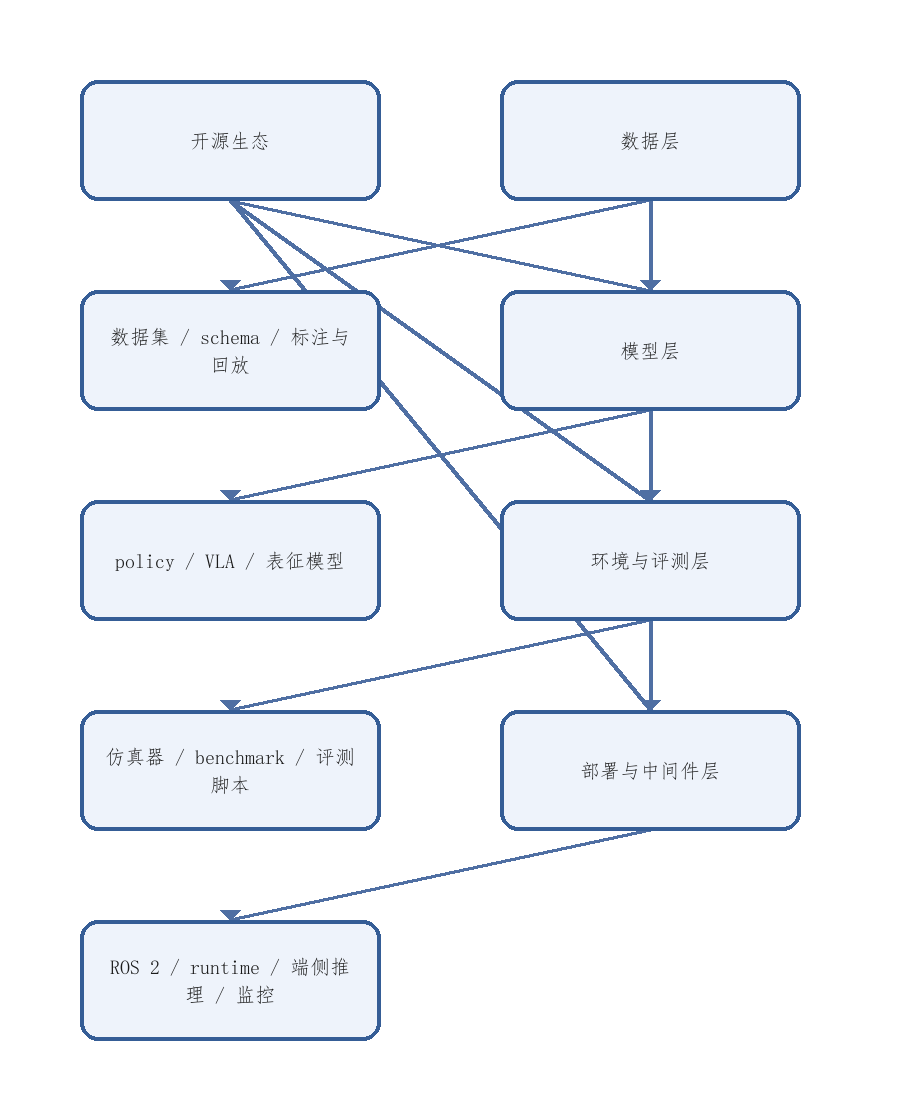
\includegraphics[width=0.9\textwidth,height=0.72\textheight,keepaspectratio]{figures/19-开源生态四层结构图.png}
\caption{19-开源生态四层结构图}
\label{fig:19-开源生态四层结构图}
\end{figure}

\chapter*{图表与案例补充}
\addcontentsline{toc}{chapter}{图表与案例补充}
\markboth{图表与案例补充}{图表与案例补充}

本章的图表与案例，不应被视为附属装饰，而应被理解为“如何把零散开源项目重新组织成学习与研究工作流”的结构化工具。对学习者来说，真正困难的往往不是知道仓库名称，而是判断一个项目位于数据、模型、环境还是部署层，并进一步识别它与自己研究目标之间缺失的工程链路。

因此，这里的补充材料应优先服务于接口关系、依赖方向、最小复现路径和失败模式分析，而不只是继续罗列项目名单。只有把这些关系显式画出来，开源生态才会从“很多仓库”转化为“可组合基础设施”。

在当前版本中，\texttt{\detokenize{图 19-1 开源生态四层结构图}} 已承担分层结构说明；19-代表性开源项目对照表 与 \texttt{\detokenize{表 19-1 开源生态四层对照表}} 则分别负责“项目级横向对照”与“生态层级定位”。

“从开源代码到最小复现实验”的路径，最好被理解成一类独立的研究资产，而不只是正文中的说明句。因为这类内容天然需要同时记录环境依赖、数据准备、训练命令、评测脚本和常见失败点，若只停留在报告叙述层，会很快丢失可复用性。因此，本章与 \path{research/}、\path{code/} 的连接并不是附属关系，而是开源章节真正能够服务后续实验工作的关键接口。

目前这章已经可以配合 19-开源生态四层对照表 和 19-代表性开源项目对照表 一起读。前者负责回答“开源生态分几层”，后者负责回答“具体项目在这几层中的什么位置、适合拿来做什么”。这样后续补项目时，就不容易重新退化成仓库名单。

\chapter*{表 19-1 开源生态四层对照表}
\addcontentsline{toc}{chapter}{表 19-1 开源生态四层对照表}
\markboth{表 19-1 开源生态四层对照表}{表 19-1 开源生态四层对照表}

\begingroup
\small
\begin{xltabular}{\textwidth}{YYYYY}
\toprule
层级 & 主要对象 & 关键问题 & 代表性项目/资产 & 主要局限 \\
\midrule
\endfirsthead
\toprule
层级 & 主要对象 & 关键问题 & 代表性项目/资产 & 主要局限 \\
\midrule
\endhead
数据层 & 采集、清洗、格式标准化、回放 & 数据是否对齐、可回流、可复现 & LeRobot、Open X-Embodiment、本地日志工具链 & 数据协议不统一、失败样本常不足 \\
模型层 & 感知 backbone、policy、VLA、world model & 输入输出接口是什么、动作表示是什么 & OpenVLA、Diffusion Policy、ACT & 模型可复现不等于可部署 \\
环境层 & 仿真器、benchmark、任务脚本、评测协议 & 奖励什么能力、忽略什么能力 & Isaac Sim、Habitat、MuJoCo、Gazebo & 平台差异导致结果难横比 \\
部署层 & ROS/中间件、端侧推理、监控告警、回放 & 能否稳定运行、可否诊断和回退 & ROS 2、edge runtime、monitoring stack & 开源资产常最薄、最难维护 \\
\bottomrule
\end{xltabular}
\endgroup

\chapter*{表 19-2 代表性开源项目对照表}
\addcontentsline{toc}{chapter}{表 19-2 代表性开源项目对照表}
\markboth{表 19-2 代表性开源项目对照表}{表 19-2 代表性开源项目对照表}

\begingroup
\small
\begin{xltabular}{\textwidth}{YYYYYY}
\toprule
项目 & 所在层 & 主要定位 & 输入输出接口关注点 & 更适合的使用阶段 & 主要局限 \\
\midrule
\endfirsthead
\toprule
项目 & 所在层 & 主要定位 & 输入输出接口关注点 & 更适合的使用阶段 & 主要局限 \\
\midrule
\endhead
OpenVLA & 模型层 & 开源 VLA 对照点 & 图像 / 语言 / 状态到动作接口 & 研究对照、接口理解、复现实验 & 离真实部署仍有明显系统差距 \\
LeRobot & 模型层 / 工具层 & 低门槛机器人学习与社区工作流 & 数据格式、训练调用、基础 policy 接口 & 学习、快速实验、社区复现 & 不能直接代表高复杂度生产级系统 \\
Open X-Embodiment & 数据层 & 跨平台机器人数据组织 & 跨机器人数据协议与样本组织 & 数据理解、基础模型训练前置 & 平台间动作和语义对齐仍然困难 \\
Diffusion Policy & 模型层 & 生成式动作学习基线 & 观测窗口到 action sequence / chunk & 动作建模研究、基线比较 & 部署时延与闭环恢复问题仍需额外系统补足 \\
ACT & 模型层 & 动作 chunking 路线代表 & 感知 + 状态到 chunked action & 操作策略基线、动作表示比较 & 需要结合系统约束解释其实用边界 \\
Habitat & 环境层 & embodied AI / 导航环境 & 环境实例化、任务 episode、评测协议 & 导航、场景交互、benchmark 研究 & 与真机接触和执行约束仍有距离 \\
Isaac Sim & 环境层 / 平台层 & 高保真仿真与平台生态 & 仿真、数据生成、训练-部署衔接 & sim2real、平台型开发工作流 & 平台依赖较强，不能自动等于真机闭环 \\
ROS 2 & 部署层 & 机器人中间件与系统总线 & 模块通信、QoS、日志、状态流 & 系统集成、部署、调试 & 不直接提供高层智能能力，需要与模型栈耦合 \\
\bottomrule
\end{xltabular}
\endgroup

从维护方法上看，后续新增开源项目时，建议先查 开源生态与工具链论文清单，再判断是否需要进入 19-代表性开源项目对照表 或 \path{data/processed/开源生态分层-v0.0.csv}。
